\section{Background}
The power to obtain enough information to detect possible trends of influenza seasons depends on successful integration between a multitude of different participants. Automatic extraction and processing of data is paramount for efficient analysis and gives a solid basis for an autonomous pathological detection system. Scalability is important in merging new relevant datasets as they become available in an ever-growing societal infrastructure. This proposed technology would become an influential part of a bigger foundation intertwined with a robust knowledgeable and organizational means to mobilize assets in order to respond to possible outbreaks as or even before they start.
\newline \\
Influenza is an exceedingly contagious viral infection which gives high fever, general pain, and respiratory symptoms\cite{fhi_sykdommer}. An estimated five to ten percent of the population becomes infected during a yearly winter season. The virus is especially dangerous to the elderly and to pregnant people from the second-trimester. Annually between the months of December and April people of the northern hemisphere are struck by influenza epidemics. Since this is a seasonal occurrence mitigation or even elimination of the effects are a priority and thus observation and research is initiated. From a historical perspective, it is known that influenza can have overwhelming destructive consequences if left freely to ravage the population. The last three larger pandemics were the Asian flu of 1957, the flu of 1968 which originated in Hong Kong and the H1N1 (swine flu) virus of 2009, which respectively claimed the lives of 1.1 million, 1-4 million and 284500 people \cite{potter2001history}. The virus mutates often which proves immunization by a vaccine to be a seasonal effort. Infection happens via droplets in the air inhaled, and even a small exposure expands to an all-out blitz which the immune system is forced to engage.

\section{Objectives}
This thesis describes a plausible examination of the viability of monitoring, collecting and analyzing relevant urban true-time data for a self-sufficient influenza seasonal recognition system. The management of seasonal influenza outbreaks is handled by public health officials and epidemiologists with the use of the national surveillance system provided by the Norwegian Institute of Public Health (NIPH)\cite{niph}. The Norwegian Syndromic Surveillance System (NorSySS) collects influenza-like illnesses (ILI) from general practitioners (GPs)\cite{NorSySS}, figure \ref{fig:norsyss} shows a diagram of their process. These provide the means to monitor current influenza seasons with delay and as a basis to survey urban real-time datasets. These subsystems compose the complete Norwegian influenza surveillance system, but they are not able to provide an expeditious real-time overlook. Typically the delay is over a week because it relies on clinical reports and laboratory endeavors, these limited mechanisms to acquire updated information on societal functions and integrity creates the need for a more agile source of investigating possible influenza outbreaks in terms of temporal geospatial information. This, in turn, would enable a more reactionary effort against epidemics, and this thesis examines this possibility.

\begin{figure}[h]
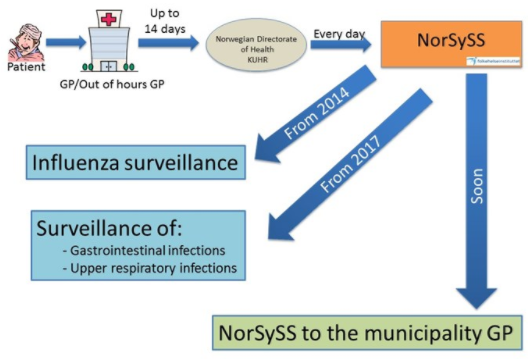
\includegraphics[width=16cm]{NorSySS_diagram}
\centering
\caption{NorSyss's process}
\label{fig:norsyss}
\end{figure}

The main suggestion of this thesis is as influenza develops it reveals subtle patterns in societal behaviors that is detectable through a variety of mediums, e.g urban datasets from sewage, public transportation, medicinal purchases, recreational habits, social media and other such sources of public information. With this suggestion, a tool to collect urban spatial datasets is needed and to present and visualize this information to best divulge the effect of the viral composition. The datasets used in this thesis is explained more in chapter 3, they consist however of the NIPH ILI and virus observations, the different datasets from the NPRA showing traffic patterns, social media of Twitter reporting symptoms directly from possible Norwegian patients and two public transportation providers of the cities Stavanger and Oslo. Unfortunately more datasets could not be obtained within the time-scope of this thesis, but nonetheless, they provide a solid basis for examination and development.

\section{Outline}
The thesis is structured into seven chapters.
\newline \\Chapter 2 describes related works of what others have found useful as tools and other proven effective measurements.
\newline \\Chapter 3 marks out in detail the datasets used by this project, describes and give an explanation to relevance, challenges, limitation, and rewards.
\newline \\Chapter 4 outlines the implementation and graphical results of the datasets used in chapter 3.
\newline \\Chapter 5 shows the overall results.
\newline \\Chapter 6 discusses the results.
\newline \\Chapter 7 concludes the thesis, discusses constraints and possible future work as well as other suggestions.